\section{Introduction}
\label{sec:introduction}

% state the learning objective 
The objective of this laboratory assignment is to study a circuit with four elementary meshes and eight nodes. 
This circuit contains an independent voltage source $V_a$, an independent current source $I_d$, 
a voltage source dependent from a current $V_c$ and a current source dependent from a voltage $I_b$.
Besides this, it has seven resistors, $R_1$, $R_2$, $R_3$, $R_4$, $R_5$, $R_6$ and $R_7$. The circuit can be seen in Figure~\ref{fig:Circuit}.\\
In Section~\ref{sec:analysis}, a theoretical analysis of the circuit is
presented, using the mesh method and the node method, in Octave. In Section~\ref{sec:simulation}, the circuit is analysed by
simulation using ngspice, and the results are compared to the theoretical results obtained in
Section~\ref{sec:analysis}. The conclusions of this study are outlined in
Section~\ref{sec:conclusion}.

\begin{figure}[h] \centering
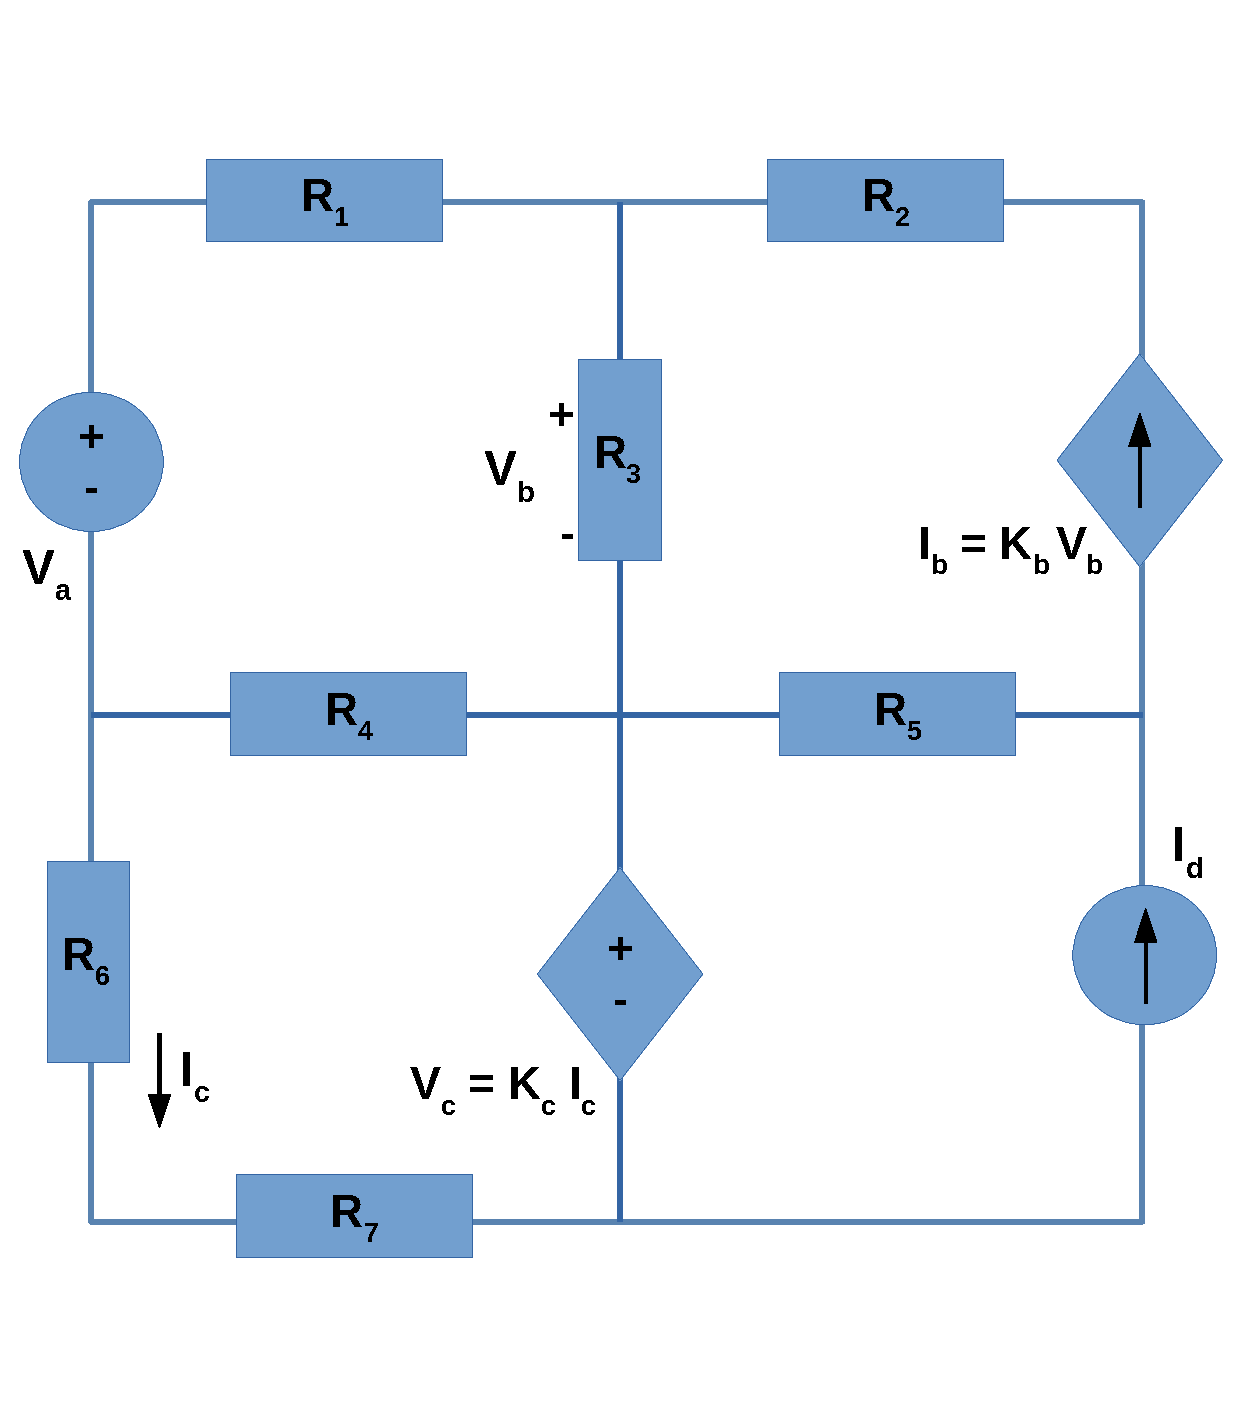
\includegraphics[width=0.6\linewidth]{Circuit.pdf}
\caption{Circuit containing voltage sources, current sources and resistors.}
\label{fig:Circuit}
\end{figure}

